\chapter{Stand van zaken} \label{ch:stand-van-zaken}

% Tip: Begin elk hoofdstuk met een paragraaf inleiding die beschrijft hoe
% dit hoofdstuk past binnen het geheel van de bachelorproef. Geef in het
% bijzonder aan wat de link is met het vorige en volgende hoofdstuk.

% Pas na deze inleidende paragraaf komt de eerste sectiehoofding.
Om growth hacking te kunnen kaderen moet men begrijpen waar het begrip van komt en hoe het ontstaan is. De bron van growth hacking ligt in bij marketing, digitale marketing, influencer marketing enz. In de volgende paragrafen zullen deze begrippen duidelijk gemaakt worden en op het einde van dit hoofdstuk zal er een concrete definitie gevormd worden over growth hacking.

\section{Wat is marketing?} \label{sec:marketing}
\begin{quote}
	``Alles wat een bedrijf doet om de verkoop van producten te bevorderen.``, definitie van marketing uit woorden.org
\end{quote}
\begin{quote}
	``The action or business of promoting and selling products or services, including market research and advertising.``, definitie van marketing uit dictionary.org
\end{quote}
\begin{quote}
``Elke activiteit die consumenten en producenten met elkaar verbindt.``, een omschrijving van marketing.
\end{quote}

Die laatste omschrijving is zeer interessant omdat het duidt op wat marketing inhoudt. Het is niet enkel advertenties, het gaat ook over community management, brand image, ... en zoveel meer. Community management is zo belangrijk geworden dat vele bedrijven hier een aparte functie voor hebben. Deze functie houdt vooral de communicatie tussen het bedrijf en de klanten op sociale media in. 

Van communicatie tussen consument en producent tot promotie van een product richting de consument en alles ertussen, dat is waar marketing voor staat.

Marketing kan men ook uitleggen aan de hand van de marketingmix (4 P's), die E Jerome McCarthy in 1960 ontwikkelde om marketing te verduidelijken. Deze 4 P's staan in connectie met elkaar en een aanpassing kan zorgen voor een volledig nieuwe marketing mix.~\autocite{Forsey2019}

\begin{itemize}
	\item Product
	\item Prijs
	\item Plaats
	\item Promotie
\end{itemize}

De marketingmix wordt gebruikt om het marketingbeleid van een organisatie te beschrijven. 

\subsection{Product} \label{sec:marketing-product}
Deze eerste P duidt zowel een product als dienst aan. Een bedrijf moet de nood of wens van een klant voldoen. Het product dient een meerwaarde te bieden voor de klant. Binnen marketing is het belangrijk dat het product goed en volledig is. Van design tot verpakking en alle services die er bij komen.
 
\subsection{Prijs} \label{sec:marketing-prijs}
"Wat is de prijs dat onze doelgroep wil betalen voor ons product?". Dat is de belangrijkste vraag dat men eerst moet stellen voordat er tal van berekeningen gemaakt worden. De juiste kostprijs bepalen zodat het bedrijf winstgevend kan zijn. Het gaat over prijsbepaling en strategie, maar ook kortingen.

Een opvallende trend in bij webshops en andere web platformen is dat er vaak korting is op veel producten. Het product is steeds goedkoper dan de ``adviesprijs``, dit is een manier om psychologische prijzen in te zetten. Een andere strategie is de prijs goedkoper te laten aanvoelen, in plaats van 10 euro kan men 9,99 vragen voor hetzelfde product~\autocite{InternetMarketingUniversiteit2016}. Dit heet ``Charm pricing``, het verschil in prijs is miniem. De consument zal eerder het product kopen dat goedkoper is dan de adviesprijs en begint met een lager getal (door de 99 cent bijvoorbeeld), dan het product dat 10 euro kost en niet goedkoper is of blijkt te zijn.

\subsection{Plaats} \label{sec:marketing-plaats}
Plaats dient een antwoord te geven op de gehele distributie van het product. "Op welke manier komt de dienst of het product bij de klant?". Vroeger was dit meestal via een verdeler die het product aan verschillende winkels levert. Tegenwoordig, door het internet, is het heel interessant geworden om de "middleman", de tussenpersoon, uit te schakelen. Bij Secret Lab is dit bijvoorbeeld 1 van hun troeven waarmee ze uitpakken op hun website. Ze verklaren de lage kost van hun hoge kwaliteit stoelen door het uitschakelen van de tussenpersoon. Het bedrijf levert de stoel vanuit hun kantoor naar de deur van de klant, bij wijze van spreken. 

\subsection{Promotie} \label{sec:marketing-promotie}
Dit wordt ook wel marketingcommunicatie genoemd. Dit is waar men meestal aan denkt wanneer iemand marketing vermeld.

Promotie maken voor je product, er voor zorgen dat men weet wat je bedrijf doet of verkoopt. Ook het imago van het bedrijf is hier onderdeel van.

Enkele promostrategieën~\autocite{marketingscriptie.nl2018}:
\begin{itemize}
	\item Reclame (internet, krant, televisie)
	\item Public Relations (bijvoorbeeld sponsoring)
	\item Plaats (acties)
	\item Persoonlijke verkoop (face-to-face, telefonisch, ...)
\end{itemize}

\section{Invloed van de digitalisering op marketing} \label{sec:digitalisering-marketing}
De digitalisering heeft een grote invloed gehad op de manier waarop bedrijven aan marketing doen. Er is een nieuwe tak binnen marketing ontstaan: digitale marketing. 

Hiervoor bestaan nu ook nieuwe jobs, de all-around digital marketeer kan op z'n eentje de marketing doen van een klein bedrijf. Grote bedrijven hebben vaak een specialist in SEO (Search Engine Optimization), die zorgt ervoor dat de website van het bedrijf makkelijk gevonden kan worden via populaire zoekmachines zoals Google en Bing. Naast een SEO specialist bestaat er vaak een community manager die via sociale media direct contact heeft met de klanten. Google en Facebook advertising kunnen door aparte teams onderhouden worden. Verder bestaan er ook ``lead generator``-experts, die via verschillende regels de ideale manier kunnen vinden om potentiële klanten binnen te halen.

\section{Nieuwe trends binnen marketing} \label{sec:nieuwe-trends-marketing}
Nu dat digitale marketing een zekere maturiteit heeft en dat zo wat alle grote bedrijven aan digitale marketing doen, ontstaan er natuurlijk nieuwe trends. 

\subsection{Influencer marketing} \label{sec:influencer-marketing}
Influencer marketing is hier één van. Zoals~\textcite{Pieters2018} aangeeft in zijn bachelorproef~\citetitle{Oord2014} is Instagram een populair en efficiënt platform om aan influencer marketing te doen. 

Een influencer is een persoon of groep personen die een meer dan gemiddeld potentieel hebben om anderen te beïnvloeden doordat zij veel communiceren en zich centraal bevinden in een (sociaal) netwerk.~\autocite{Pieters2018}

Bedrijven kunnen deals sluiten met influencers zodat ze het product of de service van het bedrijf promoten, bijvoorbeeld via een post op Instagram. Dit is veel persoonlijker dan een generieke advertentie via een digitaal medium zoals Google Adwords, Facebook Ads (hier hoort Instagram ook bij) of dergelijke. Vaak hebben influencers een bepaalde doelgroep, wanneer deze perfect aansluit bij het bedrijf zal het product waarschijnlijk ook goed ontvangen worden door de volgers van de influencer. Hierdoor kan één post een heel positieve impact hebben op de omzet van het bedrijf. De influencer wordt vaak vergoed door een geldsom, soms kan dit ook een verblijf in het buitenland zijn voor bepaalde activiteiten. Door het bedrijf wordt de reis, het verblijf en de activiteiten dan betaald. Beide partijen komen er op deze manier beter uit.


\subsection{Content marketing} \label{sec:content-marketing}
Content marketing is een belangrijk fenomeen in de digitale marketing wereld. Het behalen van een goede score bij zoekmachines ligt voor een groot deel bij het schrijven van goede content. Bij het schrijven van deze 'goede content' moet er steeds rekening gehouden worden met de belangrijke keywords die rond het onderwerp vaak gezocht worden. 

In 2014 schreef Bob Oord van RIFF Content Marketing over ~\citetitle{Oord2014}. In dit artikel bespreekt hij de verschillende rollen die de marketingafdeling in 2020 zou bevatten. Hij spreekt over heel veel rollen, maar deze kunnen ondergebracht worden onder enkele functies of binnen een klein bedrijf 1 functie: de contentmarketeer. 

\subsection{Guerrillamarketing} \label{subsec:guerrillamarketing}
Guerillamarketing wordt vaak samen gebruikt met ``Zero Budget Marketing`` en growth hacking. Het is een marketingtechniek waarbij men met beperkte middelen een groot resultaat wil behalen. De focus ligt op het halen van veel (media-)aandacht tot het merk of product. Men wil een groot publiek bereiken en op die manier er voor zorgen dat het publiek vertrouwd geraakt met de merknaam of het product.

Dit gebeurt door bijvoorbeeld ludieke acties of stunts die heel snel en efficiënt zijn in het bereiken van een groot publiek. 

Growth hacking kan men onder de term Guerillamarketing plaatsen, want in essentie wil men via growth hacking ook met beperkte middelen een groot resultaat behalen.

Enkele voorbeelden van gueriallamarketing:
 
\begin{itemize}
	\item Reverse graffiti: selectief schoon maken van een muur 
	\item Virale marketing: posts delen via sociale media die de ontvangers opnieuw gedeeld worden
	\item Internetmemes: door het creëren van een grappige afbeelding of post op sociale media kan deze viraal gaan
	\item Flashmob: op een openbare plek een (grote) groep mensen laten samenkomen en iets ongebruikelijks laten uitvoeren dat achteraf weer snel uiteenvalt
	\item Posters plakken: soms op illegale plaatsen, om extra aandacht te trekken
\end{itemize}

\begin{figure}[h!]
	
\includegraphics[width=55mm]{img/reverse-graffiti.jpg}
	\centering
	\caption{Reverse graffiti. \textcopyright  Lisa Müllerauh}
	\label{fig:defGrowthHacker}
\end{figure}

\begin{figure}[h!]
	
\includegraphics[width=\linewidth]{img/dbrand-internetmeme.jpg}
	\centering
	\caption{Internetmeme van dbrand. Ze spelen in op een recent memeformaat en passen het toe op hun eigen product(en). Zo kunnen ze met amper budget, enkel owned en earned media, een heel groot publiek laten weten dat hun product bestaat.}
	\label{fig:defGrowthHacker}
\end{figure}

\section{Wat is growth hacking?}
\label{sec:wat-is-growth-hacking}
Growth hacking is ook een nieuwe trend binnen marketing die vaak onduidelijkheid met zich mee brengt. Dus dan komt de vraag: wat is growth hacking nu exact?

Nicholas D’hondt beschrijft growth hacking in een artikel van~\textcite{Birdhouse2019} als een mindset van heel veel experimenteren en constant op zoek gaan naar nieuwe kanalen die kunnen zorgen voor groei. 

Het gaat om zoveel mogelijk mensen binnen je doelgroep te bereiken, zo kan je als bedrijf met (zeer) weinig geld een groot resultaat behalen. 

Sommige bedrijven willen een bepaalde boodschap verspreiden, andere willen enkel hun merknaam naar buiten krijgen. Het draait steeds om groeien, in welk specifiek gebied dat je wil groeien moet je voor ieder experiment steeds definiëren. Zo kan je leren uit het experiment, het is namelijk niet de bedoeling dat er zomaar uit het niets wordt geëxperimenteerd. Er zullen veel experimenten falen en het is de bedoeling dat er steeds iets uit geleerd kan worden. Dit is mogelijk door op voorhand goed te weten wat het doel is, ook moet er achteraf genoeg documentatie voorzien worden van het experiment. Waarom het doel al dan niet behaald werd kan veel verduidelijking geven en kan je in de juiste richting duwen.

Wanneer er kleine realistische (en S.M.A.R.T.) doelen gezet worden zorgt dit ook een goed mentaal effect, je komt in een soort "flow" terecht, veel momentum door het steeds behalen van de doelen. Dit zorgt voor veel motivatie en het creëert ruimte om te experimenteren. Het S.M.A.R.T. principe is een afkorting en staat voor:
\begin{itemize}
	\item Specifiek - Is de doelstelling eenduidig?
	\item Meetbaar - Onder welke (meetbare/observeerbare) voorwaarden of vorm is het doel bereikt?
	\item Acceptabel - Zijn deze doelen acceptabel voor de doelgroep en/of het management?
	\item Realistisch - Is het doel haalbaar?
	\item Tijdsgebonden - Wanneer (in de tijd) moet het doel bereikt zijn?
\end{itemize}

Bijvoorbeeld: ``Over vijf jaar wil ik projectmanager zijn, verantwoordelijk voor ICT-projecten van 100.000 tot 1.000.000 euro.`` \textcopyright carrieretijger.nl

In de podcast van ~\textcite{fizzle.co2015}~\citetitle{fizzle.co2015} wordt growth hacking aanzien als een buzzword, wat op dit moment zeker wel waar is. Ondanks dat de term buzzword wordt gebruikt, betekent dit niets slecht. Ze erkennen ook de mooie kanten van growth hacking zoals de creativiteit van growth hackers (of growth hacking teams). Ze worden verplicht om creatief te zijn, omdat er geen geld is. 

De slechte kant van growth hacking is volgens de podcast van~\autocite{fizzle.co2015} dat sommige mensen het zien als een manier om het systeem te "hacken", te misbruiken, om zo veel aandacht tot het product of bedrijf te krijgen. Dat is natuurlijk geen lange termijn strategie.

Een goed voorbeeld van growth hacking is het experimenteren van een schaalbare aanpak waarbij gebruikers zelf zorgen voor meer gebruikers. In een ideale situatie heb je zo'n goed product dat mensen er gek van zijn en dat deze ``viral factor`` ontstaat. Als men heel tevreden is van het product zal het zichzelf wel verspreiden. Groupon heeft het op deze manier aangepakt en is een goed voorbeeld hiervoor.

Opvallend is ook dat veel growth hacks een ``build-in expiration date`` hebben. Dat wil zeggen dat ze na een tijdje niet meer zullen werken. Een goed voorbeeld is Facebook advertenties: vroeger kon je dit gebruiken als growth hack. Je kon door je aanwezigheid op Facebook heel veel mensen binnen je doelgroep bereiken. Op dit moment wordt het niet meer gezien als growth hack, doordat de keywords waarop men wil adverteren te duur zijn geworden.

\begin{figure}[h!]
	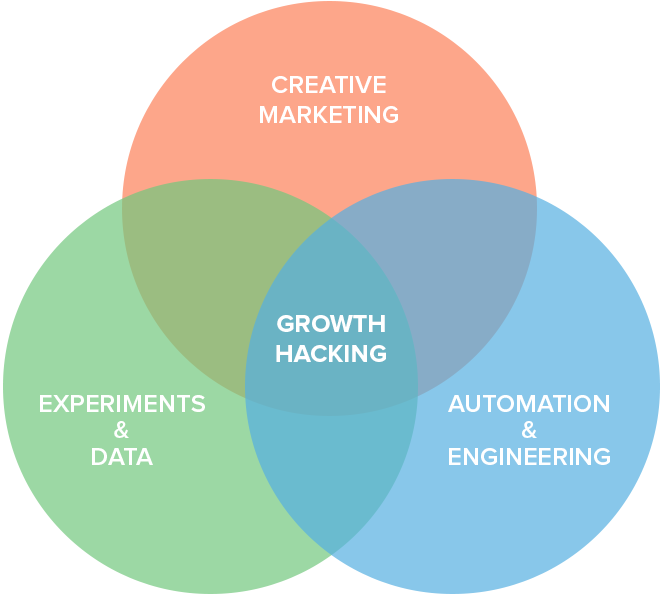
\includegraphics[width=\linewidth]{img/growth-hacking-essential-parts.png}
	\centering
	\caption{Essentiële onderdelen van growth hacking. Bron: \autocite{Rosado2018}}
	\label{fig:partsGrowthHacking}
\end{figure}

\subsection{Voorbeelden van growth hacks} \label{sec:growth-hacking-voorbeelden}
\begin{itemize}
	\item \textbf{Airbnb}: Gebruik maken van de community van Craigslist\footnote{Craigslist is een online platform dat voornamelijk in de Verenigde staten gebruikt wordt. Het wordt gebruikt om vacatures, woningen, cv's en dergelijke op te plaatsen.}. Airbnb stuurde e-mails naar de gebruikers van Craigslist die hun woning op dat platform geplaatst hadden met het verzoek om deze ook op Airbnb te plaatsen. Het werkte ook in de omgekeerde richting: vanuit Airbnb kon je met 1 klik je woning op Craigslist plaatsen (met een link terug naar Airbnb natuurlijk). 
	\item \textbf{Dropbox}: een referral programma\footnote{Wanneer je iemand doorverwijst naar de service of een product van een bedrijf en je hiervoor vergoed wordt.} dat voor beide partijen voordelig is. Wanneer men iemand succesvol kon laten registreren, via een persoonlijke link, kregen beide partijen gratis opslag op Dropbox.
	\item \textbf{Hotmail}: De eerste growth hack, ``PS: I Love You``. Onderaan iedere e-mail werd er één lijn toegevoegd: ``PS: I love you. Get your free e-mail at Hotmail.``. Waarbij Hotmail een link was naar de registratiepagina. 
	\item \textbf{Spotify}: Door de nauwe samenwerking met Facebook kon je steeds zien naar welke liedjes je vrienden luisterde op Spotify. Zo ontdekte duizenden mensen het platform en ze konden eenvoudig een account aanmaken door in te loggen via Facebook. Spotify gebruikt nu nog steeds growth hacks, zoals de verschillende partnerships met bedrijven zoals Facebook Messenger, Tinder, enz. Het is makkelijker dan ooit om een liedje door te sturen naar je vrienden, via Spotify.
\end{itemize}

\subsection{Growth hacking binnen een bedrijf} \label{sec:growth-hacker-functie}
Een growth hacker is half marketeer en half ingenieur, zoals vermeld in het onderzoeksvoorstel en geïllustreerd door de afbeelding hieronder.
\begin{figure}[h!]
	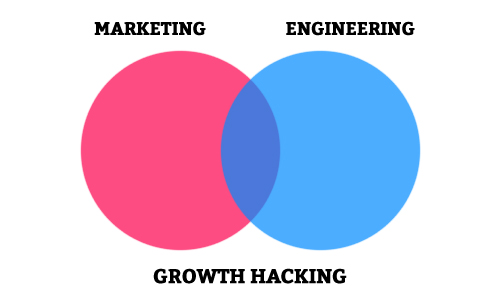
\includegraphics[width=\linewidth]{img/growth-hacker-definition.jpg}
	\centering
	\caption{Definitie van growth hacking, "Growth hacking as a fusion of two fields"  (Brody 2013, geciteerd 13.05.2016)}
	\label{fig:defGrowthHacker}
\end{figure}

In het artikel van The Birdhouse~\citetitle{Birdhouse2019} vertelt Nicholas dat growth hacking moet leven in de hele organisatie. Er moet een team gecreëerd worden met mensen uit verschillende branches van het bedrijf: developers, entrepreneurs, marketing en sales zetten we bij elkaar. In deze situatie is er niet één growth hacker, er kan wel iemand zijn die alle mensen bij elkaar brengt en het concept van growth hacking uitlegt. Als we die persoon als growth hacker zien is hij of zij eerder een soort coach die het team zal helpen om rond growth hacking te brainstormen.

Bij kleinere bedrijven kan het zijn dat er één growth hacker is, deze zal dan het profiel hebben van een marketeer en ingenieur en zal doorheen het bedrijf informatie moeten vergaren. Met al die informatie kan hij of zij experimenten bedenken of collega's aanspreken en hun ideeën implementeren of deze verwerken en doorgeven aan de developers of andere marketeers. 

In de podcast,~\citetitle{fizzle.co2015}, van~\autocite{fizzle.co2015} spreken ze over een ingenieur die aan marketing doet. Dat is het profiel van een growth hacker volgens hun. Ze zien het zo omdat een ingenieur vaak een ``data-driven`` aanpak heeft, denken vanuit data om zo experimenten in eerste instantie te creëren en vervolgens ook bij te sturen. 

Het is ook belangrijk om steeds feedback te vragen aan je collega's en natuurlijk ook de klanten, zo kan er samen aan het product gewerkt worden.

\section{Wat is het verschil met guerrillamarketing?} \label{sec:verschil-met-guerrillamarketing}

In~\citetitle{fizzle.co2015}~\autocite{fizzle.co2015} wordt er dieper ingegaan op het bredere concept van ``Zero Budget Marketing``. Ze praten over growth hacking als een tactiek binnen guerillamarketing. 

Guerillamarketing is eerder ``old-school`` en gaat ook breder dan growth hacking. Bij growth hacking ligt de focus op het digitale, dus online verschillende experimenten uitvoeren. Het is een hele nieuwe dimensie waarbij men dus eerder denkt aan growth hacking en niet guerillamarketing.

Zoals in \ref{subsec:guerrillamarketing} uitgelegd is guerillamarketing een marketingtechniek waarbij men vooral fysieke acties zal ondernemen om groei of naambekendheid te realiseren. 

\section{Hoe begin je aan growth hacking?} \label{sec:hoe-growth-hacking}
 
Zoals eerder vermeld draait growth hacking om de experimenten die je uitvoert, maar hoe begint men er aan?

Men kan eerst een audience (of groep mensen die je volgen) opbouwen, zoals @portland heeft gedaan op Instagram, en achteraf een bedrijf opstarten rond je bestaande audience, zoals @portlandgear. Het zijn 2 Instagram-accounts van dezelfde persoon, hij of zij zag dat er interesse was voor producten in verband met portland. Daardoor was het creëren van een webshop een zeer goed idee, toen was @portlandgear geboren. Via de eerste Instagram-account worden er posts gezet met producten van de tweede account.

Het is een voorbeeld van hoe je met growth hacking aan de slag kan. Natuurlijk lopen lang niet alle growth hacks op die manier. Het gaat ook helemaal niet heel snel of plots, je moet bijvoorbeeld in zo'n Instagram-account veel tijd steken en zorgen dat het interessant is om te volgen. Als dat niet het geval is gaat er niemand de account volgen en zijn er dus geen potentiële klanten.

Naast het Instagram voorbeeld zijn er enkele algemene regels waar men zich aan kan houden voor het opstellen van goede experimenten. 

\begin{itemize}
	\item Data is key: alles moet opgeslagen worden, dus alle tracking-tools moeten werken en getest zijn
	\item Zodra alles voldoende kan opgevolgd worden kan men beginnen denken over het doel van het eerste experiment. Het is belangrijk om een duidelijk, S.M.A.R.T. doel te hebben, zoals eerder vermeld.
	\item Dan begint men met het zoeken van de personas die men wil bereiken én waar deze te vinden zijn. Welke kanalen er best gebruikt kunnen worden om deze personas te vinden.
	\item Nadat het experiment is uitgevoerd kunnen er via de tracking-tools veel vragen beantwoord worden. Of het aantal bezoekers op de website al dan niet gestegen is, of de omzet gestegen is, wat het resultaat is op sociale media. Enzovoort... 
\end{itemize}

In het volgende hoofdstuk wordt er dieper ingegaan op hoe je growth hacking kan toepassen op een bedrijf. Dit wordt bevestigd door verschillende mensen in het werkveld, die geïnterviewd worden met gerichte vragen rond het onderwerp.

